
\chapter{Light Field Photography}

The propagation of the light rays in the 3D space can be completely described by a 7D continuous function $R(\theta,\phi,\lambda,\tau,V_x,V_y,V_z)$, where $(V_x,V_y,V_z)$ is a location in the 3D space, $(\theta,\phi)$ are propagation angles, $\lambda$ is the wavelength and $\tau$ the time; this function is known as the plenoptic function and describes the amount of light flowing in every direction through every point in space an any time, the magnitude of $R$ is known as the radiance.  In an 1846 lecture entitled "Thoughts on Ray Vibrations" Michael Faraday proposed for the first time that light could be interpreted as a field, inspired by his work on magnetic fields; but the idea of a plenoptic function representing the spectral radiance distribution of rays was first proposed by Adelson and Bergen \cite{Adelson-Plenoptic}. 

\begin{figure}[h!]
\centering
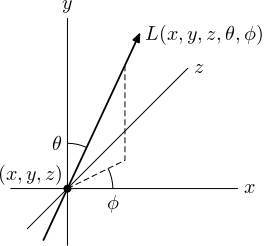
\includegraphics[width=0.5\textwidth]{./Diagrams/Plenoptic_function.jpg}
\caption{Spatio-angular parametrization of the plenoptic function for fixed $\tau$ and $\lambda$. Figure taken from Wikipedia (https://en.wikipedia.org/wiki/Light\_field)}
\end{figure}

In a more practical approach the plenoptic function can be simplified to a 4D version, called 4D Light Field or simply Light Field (abbreviated from now on as LF), denoted as the function $L$. The LF quantifies the intensity of static and monochromatic light rays propagating in half space, though this seems like an important reduction of information, this constraint does not substantially limit us in the accurate 3D description of the scene from where the light rays come from.

 There exists three tipical forms of this 4D approximation: 
\begin{enumerate}
\item The LF rays positions are indexed by their Cartesian coordinates on two parallel planes, also called the two-plane parametrization $L(u,v,s,t)$.
\item The LF rays positions are indexed by their Cartesian coordinates on a plane and the directional angles leaving each point, $L(u,v,\phi,\theta)$.
\item Pairs of points on the surface of a sphere $L(\phi_1,\theta_1,\phi_2,\theta_2)$.
\end{enumerate}

\begin{figure}[h!]
\centering
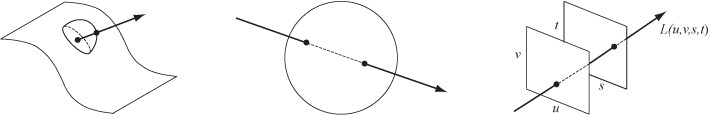
\includegraphics[width=1.0\textwidth]{./Diagrams/Light-field-parametrizations.jpg}
\caption{Three different representations of 4D LF. Left: $L(u,v,\phi,\theta)$. Center: $L(\phi_1,\theta_1,\phi_2,\theta_2)$. Right: $L(u,v,s,t)$. Figure taken from Wikipedia (https://en.wikipedia.org/wiki/Light\_field)}
\end{figure}

In this work we will centered our attention in the two plane parametrization $L(u,v,s,t)$, if you are interested in the other descriptions we recommend to see \cite{Liang}. In order to understand deeply this way of LF description, lets consider a camera with image plane coordinates $(u,v)$ and the focal distance $f$ moving along the $(s,t)$ plane. 

\begin{figure}[h!]
\centering
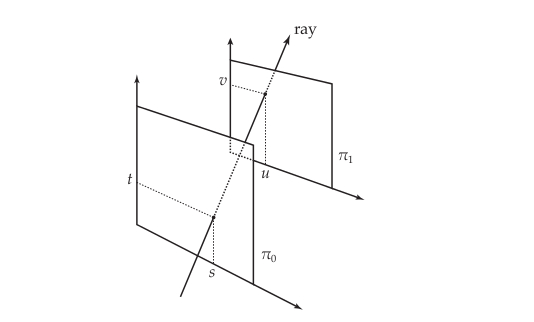
\includegraphics[width=1.0\textwidth]{./Diagrams/two-planes_param.jpg}
\caption{Graphic representation of the two plane parametrization of a single ray on the LF which is parametrized by the intersection $(s,t)$ and $(u,v)$ with planes $\pi_0$ and $\pi_1$, respectively. Figure taken from \cite{Kim-Disney} p.21}
\end{figure}

For simplicity one can constrain the vertical camera motion by fixing $s = s_0$ and moving the camera along the $t-axes$ in an straight light motion, in the section~\ref{sec:Epi-geometry} we will see that this constraint leads to an elegant geometric 3D representation of the scene called Epipolar Geometry, this multiview aquisition is refered as parallax only (HPO). Under this constraint, images captured by successive camera positions $t_1$, $t_2$,... can be stacked together, and one can also interpret each camera position as a time step.

\begin{figure}[h!]
\centering
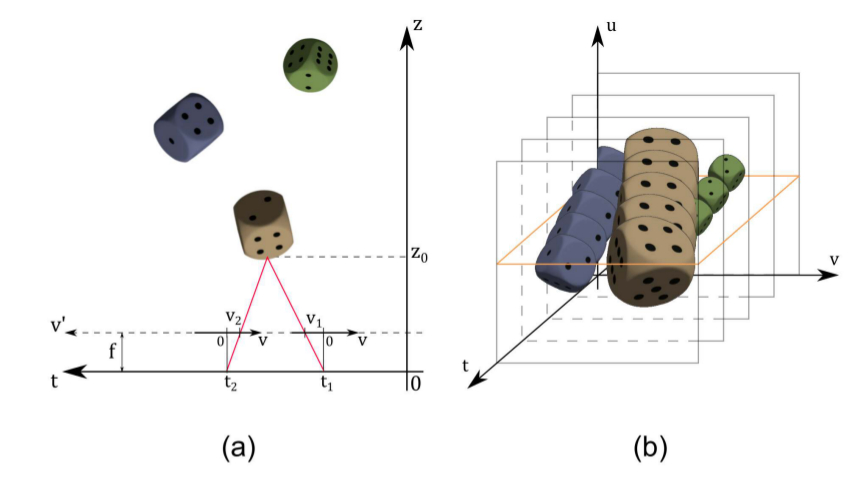
\includegraphics[width= 0.90\textwidth]{./Diagrams/images_stacked.jpg}
\caption{Stacked captured images represented in (b) from the scene setup (a). Figure taken from \cite{LF-Shearlets} p. 2}
\end{figure}

\section{Light Field Photography in the History}

For different reasons of interest for science and art capturing light fields has been an active research area for more than 110 years (the reason will be explained in detail on the section \ref{sec:LF-applications}). In 1903 Herbert E. Ives \cite{Ives} was the first to realize that the light field inside a camera can be recorded by placing a pinhole or lenslet arrays in front of a film sensor (what is know as pinhole camera). On the other hand, in 1908 the french physicist and Nobel laureate Gabriel Lippmann published two articles about something that he called \textit{photographie int\'egrale} (translated as integral photography) \cite{Lippmann} in which he describes an imaging apparatus with an arrange of small lenses on a 2D grid that are able to capture multiple images of a scene with viewpoint variations, is quite surprising that almost 110 year ago he could have the idea that modern state of the art LF aquisition systems use

\section{Epipolar Geometry, Stereo Vision and Image rectifictation}
\label{sec:Epi-geometry}

\section{Sparse aquisition of Epipolar-plane}

\section{Typical applications for the Light Field Theory}
\label{sec:LF-applications}
